% !TEX TS-program = pdflatex
% !TEX encoding = UTF-8 Unicode

% This is a simple template for a LaTeX document using the "article" class.
% See "book", "report", "letter" for other types of document.

\documentclass[20pt]{article} % use larger type; default would be 10pt

\usepackage[utf8]{inputenc} % set input encoding (not needed with XeLaTeX)

%%% Examples of Article customizations
% These packages are optional, depending whether you want the features they provide.
% See the LaTeX Companion or other references for full information.

%%% PAGE DIMENSIONS
\usepackage{geometry} % to change the page dimensions
\geometry{a4paper} % or letterpaper (US) or a5paper or....
% \geometry{margin=2in} % for example, change the margins to 2 inches all round
% \geometry{landscape} % set up the page for landscape
%   read geometry.pdf for detailed page layout information

\usepackage{graphicx} % support the \includegraphics command and options

% \usepackage[parfill]{parskip} % Activate to begin paragraphs with an empty line rather than an indent

%%% PACKAGES
\usepackage{booktabs} % for much better looking tables
\usepackage{array} % for better arrays (eg matrices) in maths
\usepackage{paralist} % very flexible & customisable lists (eg. enumerate/itemize, etc.)
\usepackage{verbatim} % adds environment for commenting out blocks of text & for better verbatim
%\usepackage{subfig} % make it possible to include more than one captioned figure/table in a single float
\usepackage{mathtools}
\usepackage{graphicx} % supports images in latex
% These packages are all incorporated in the memoir class to one degree or another...

\usepackage{graphicx}
\usepackage{subcaption}

%%% Other stuff
\DeclarePairedDelimiter\ceil{\lceil}{\rceil}
\DeclarePairedDelimiter\floor{\lfloor}{\rfloor}

%%% HEADERS & FOOTERS
\usepackage{fancyhdr} % This should be set AFTER setting up the page geometry
\pagestyle{fancy} % options: empty , plain , fancy
\renewcommand{\headrulewidth}{0pt} % customise the layout...
\lhead{}\chead{}\rhead{}
\lfoot{}\cfoot{\thepage}\rfoot{}

%%% SECTION TITLE APPEARANCE
\usepackage{sectsty}
\allsectionsfont{\sffamily\mdseries\upshape} % (See the fntguide.pdf for font help)
% (This matches ConTeXt defaults)

%%% ToC (table of contents) APPEARANCE
\usepackage[nottoc,notlof,notlot]{tocbibind} % Put the bibliography in the ToC
\usepackage[titles,subfigure]{tocloft} % Alter the style of the Table of Contents
\renewcommand{\cftsecfont}{\rmfamily\mdseries\upshape}
\renewcommand{\cftsecpagefont}{\rmfamily\mdseries\upshape} % No bold!

%%% Code syntax highliting
\usepackage{listings}
%\begin{lstlisting}[language=java]
%\end{lstlisting}

%%% graphics path \graphicspath{{./HW5}}

%%% END Article customizations

%%% nice things to keep around

% \noindent\rule{2cm}{0.4pt} 
%%% puts a small horizontal line

% \mathcal{O} 
%%% big O notation

%\begin{figure}[!htbp]
%  	\centering
%   	\begin{subfigure}[p]{0.5\linewidth}
%    	\includegraphics[width=\linewidth]{}
%   	\end{subfigure}
%\end{figure} 

%%% The "real" document content comes below...

\title{Senior Paper: The Mandelbrot Set}
\author{Liam Dillingham}
%\date{} % Activate to display a given date or no date (if empty),
         % otherwise the current date is printed 

\begin{document}
\maketitle

\section{Introduction}
The Mandelbrot Set is a set of numbers in $\!C$ that satisfy behaviors under the constrains of a given function.  While the numbers within the set, and the numbers clearly not in the set seem straight-forward, the popular interest in this set comes from the bizarre behavior of what occurs on the boundary of the set.  The behavior of what occurs on the boundary of the set seems to go on with inifinitely minute detail, and there are many videos on the internet of people exploring certain areas of this boundary to incredible precision.  What we want to do is explore some of the concepts behind this behavior, in hopes to have a better understanding of what is occuring when we look at this set.

\section{Iteration of a Function}
To \textit{iterate} a function $f$ means to take the value of the function for a given input, and pipe that value back in as an input, i.e. 
$$ f(x_0)=x_1, f(x_1)=x_2, f(x_2)=x_3 ...$$
Where $x_0$ is some sort of initial input or condition.  We can label these iterations like this: $f^{(0)}(x_0)=x_1, f^{(1)}(x_1)=x_2, ...$ Where $f^{(i)}(x_i)=x_{i+1}$.  It is worth noting that when we graph the iteration of a function, the coordinates look like this: 
$$( \ x_i, f^{(i)}(x_i)\ ) = (x_i, x_{i+1}) $$ 
The reason it is worth noting this is there are cases when $x_i = x_{i+1}$ for some point $(x_i, x_{i+1})$ that are important in understanding the construction of the Mandelbrot Set.

\section{Orbits}
In the previous section we introduced the concept of \textit{iterating} a function $f$ over an initial input $x_0$.  The \textit{orbit} of $x_0$ under $f$ is the sequence of points that result from iterating $f$ over its initial input $x_0$.  This initial input is called the \textit{seed} of the orbit. \\

There are many different kinds of orbits, but the most important one, which we will look at first, is called a \textit{fixed point}, where $f(x) = x$.  If you recall from the previous section where we mentioned the point $(x_i, x_{i+1})$, where $x_i = x_{i+1}$ for all $i$, this is a fixed point under our function. An example of fixed points under a function $f$ is the function $f(x) = x^{3}$, where the fixed points are $-1, 0, 1$, as$ f^{n}(-1)=-1$, $f^{n}(0)=0$, and $f^{n}(1)=1$ for any $n$. Remember than the $n$ "power" does not actually mean raise the function to the $n$th power, but rather \textit{iterate} the function by composing it $n$ times, i.e. $f^{n}(f^{n-1}(...f^{1}(f^{0}(x_0))..))$. \\

Fixed points may also be found geometrically by graphing the function, as well as the identity function, $y=x$.  Wherever the graph of our function intersects that line, we have a fixed point.  This is true because of what we mentioned earlier about $x_i = x_{i+1}$ for all $i$.  For example, given the function $f(x) = x^{2}$, and super-imposing the identity function $y=x$ over it, we can quickly spot the fixed orbits.

\begin{figure}[!htbp]
  	\centering
   	\begin{subfigure}[p]{0.5\linewidth}
    	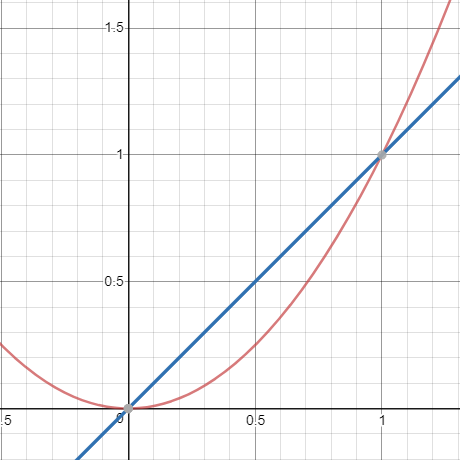
\includegraphics[width=\linewidth]{./figures/fp-1.png}
	\caption{fixed point orbits $\{0,1\}$ of $f(x)=x^{2}$}
   	\end{subfigure}
\end{figure} 

Another type of orbit is called the \textit{eventually fixed} orbit.  the orbit of some point $x_0$ is \textit{eventually fixed} if $x_0$ itself is not fixed or periodic, but some point on the orbit of $x_0$ is fixed or periodic.  For example, given the function: 
$$f^{n}(x_0)=\frac{x_0}{2^{n}}$$
Given any $x_0 \neq 0$, as $n \rightarrow \infty$, the sequence $\{ \frac{1}{2^{n}} \}$ tends towards 0.  So we can say, the orbit of $x_0$ converges to the fixed point 0, and thus is \textit{eventually fixed}. \\ 

Now, returning to our function $f(x)=x^{2}$, we can graphically analyze the orbits of a given point by tracing how the output of one iteration pipes into the input of the next iteration.  For example, let's choose a point $x_0$ such that $0 < x_0 < 1$, That is, between the two fixed points.  

\newpage
We plot our point on the $x$-axis, and apply the function $f(x)=x^{2}$ to our \textit{seed} $x_0$, which takes us up vertically to the curve.
\begin{figure}[!htbp]
  	\centering
   	\begin{subfigure}[p]{0.5\linewidth}
    	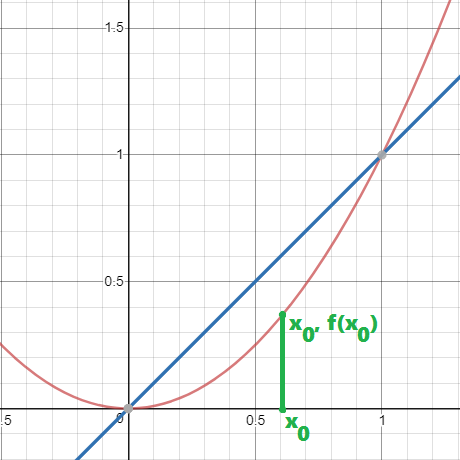
\includegraphics[width=\linewidth]{./figures/fp-2.png}
	\caption{PLACE HOLDER}
   	\end{subfigure}
\end{figure} 

Now recall that we are iterating this function, so the output, i.e. $f(x_0)$ becomes our input for our second iteration.  This is equivalent to drawing a horizontal line from the point $(x_0, f(x_0))$ to the $y=x$ line, such that we are at the point $(f(x_0), f(x_0))$.  Now we want to compute $f^{2}(x_0)$, so we need to draw a vertical line from the point $(f(x_0), f(x_0))$, to the point $(f(x_0), f(f(x_0))) = (f(x_0), f^{2}(x_0))$.

\begin{figure}[!htbp]
  	\centering
   	\begin{subfigure}[p]{0.5\linewidth}
    	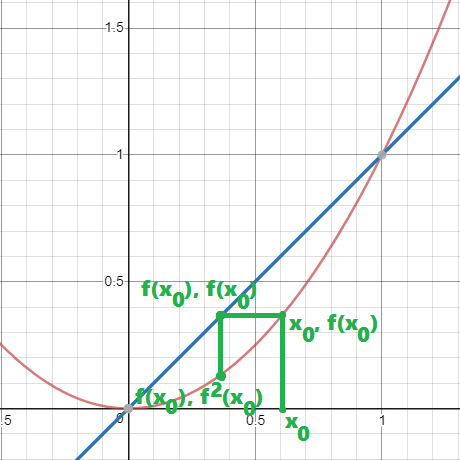
\includegraphics[width=\linewidth]{./figures/fp-3.png}
	\caption{PLACE HOLDER}
   	\end{subfigure}
\end{figure} 

By continuing this process of calcuating the point $(x_i, f(x_i)$, then drawing to the identity line to transform the output to the new input, we can find the orbit of our given \textit{seed} under our function $f$.

\begin{figure}[!htbp]
  	\centering
   	\begin{subfigure}[p]{0.5\linewidth}
    	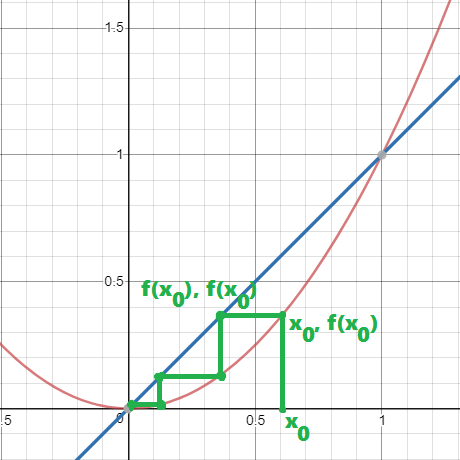
\includegraphics[width=\linewidth]{./figures/fp-4.png}
	\caption{PLACE HOLDER}
   	\end{subfigure}
\end{figure}

So we can infer from this example, that for all points $0 < x_0 < 1$, the orbit is \textit{eventually fixed}, that it converges to 0.  This concept it critical to understanding how values become accepted into the Mandelbrot Set. 

\newpage
Let's look at the same graph again, but in a different window.  Here we can see again our fixed point of 1, but this time let's choose an $x_0$ such that $x_0 > 1$. If we play the same game, plotting first $(x_0, f(x_0))$, then drawing to the $y=x$ line, and so on, we can see we have much different behavior.

\begin{figure}[!htbp]
  	\centering
   	\begin{subfigure}[p]{0.5\linewidth}
    	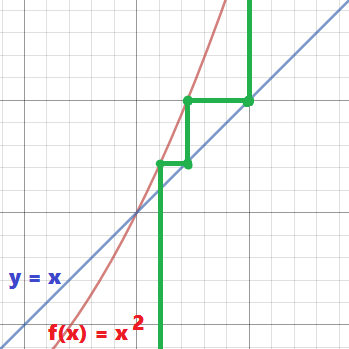
\includegraphics[width=\linewidth]{./figures/fp_1-1.png}
	\caption{PLACE HOLDER}
   	\end{subfigure}
\end{figure}

The orbit explodes, or as $n\rightarrow \infty$, the orbit diverges to infinity.  So we can see that orbits are sensitive to the initial seed, that, given a certain function, the initial condition can determine how the function behaves under iteration. \\

We can change this problem, such as, if instead of varying our seed $x_0$, we instead vary the $y$-intercept, $c$.  We can then find for what values of $c$ does the orbit given the seed $x_0 = 0$ explode.  Then our equation will look more like $f(x_0) = x_0^{2} + c$. So for $n=0$, we have $f(0)^{0} = 0^{2} + c$.  Then our first point will be $(0, c)$, our second will be
$(c, c^2 + c)$, and our third $(c^{2}+c, (c^{2}+c)^{2}+c)$ and so on. \\

So the obvious next question to ask is, for what values of $c$ do we have orbits that explode? Or rather, for what values of $c$ does the orbit converge? Let's try values of $c$ such that $0 < c < 1$, or rather, $c = 1/x$, where $x > 1$. We could constrain $x$ such that $|x| > 1$, but let's just stick to positive numbers for now. So lets begin with our seed 0, and crunch the numbers. 

$$ f^{0}(0) = (0)^{2} + 1/x$$
$$f^{1}(1/x) = (1/x)^{2} + 1/x = \frac{1}{x^{2}} + \frac{1}{x} = \frac{x^{2}+x}{x^{3}}$$.
$$f^{2}(\frac{x^{2}+x}{x^{3}}) = (\frac{x^{2}+x}{x^{3}})^{2} + \frac{1}{x} = \frac{x^{4}+2x^{3}+x^{2}}{x^{6}} + \frac{1}{x} = \frac{x^{6}+x^{5}+2x^{4}+x^{3}}{x^{7}}$$

After this the algebra becomes quite bothersome to do by hand, but it appears that the equation will converge to 0, as the equation appears to always be dominated by the $x$-term in the denominator.  But how do we prove this? Also, is it simply values of $c$ between 0 and 1? Or is the criteria something more complicated? 

\newpage
To check my intuition, I did an empirical test.  I used the R language, which, if you are unfamiliar with, is a computer programming language commonly used in statistical computing. I wrote some code to generate some evenly distributed values of $c$ and compute the behavior of their orbits for $n=50$ iterations. I tested values of $c$ such that $-3  \leq c \leq 3$, and changed $c$ by a value of 0.001 each time. After running, I plotted the points and the corresponding value after 50 iterations.

\begin{figure}[!htbp]
  	\centering
   	\begin{subfigure}[p]{0.95\linewidth}
    	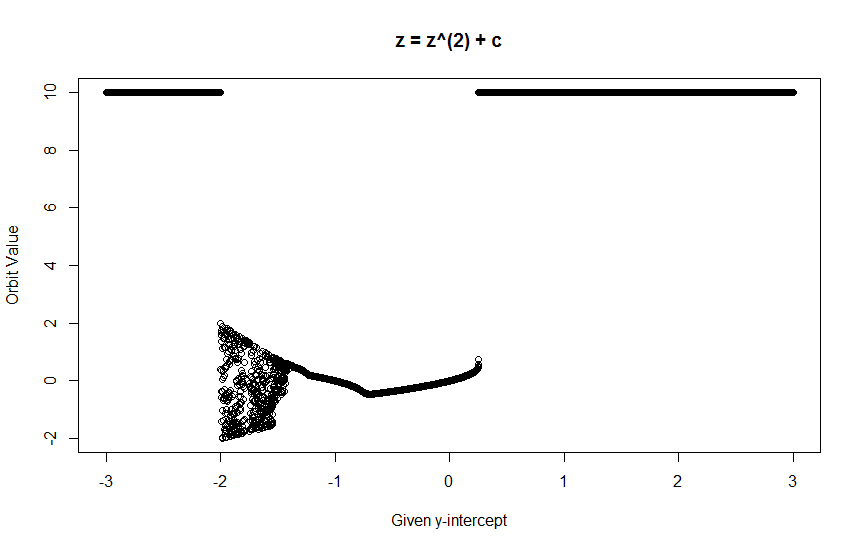
\includegraphics[width=\linewidth]{./figures/growth.png}
	\caption{PLACE HOLDER}
   	\end{subfigure}
\end{figure}

I put a condition on the graph, such that if the absolute value of the orbit was $\geq 10$, positive, or negative infinity, to set the value automatically to 10.  On the right side, the values seem to explode pretty quickly after what appears to be 0.25, but on the left the behavior is more interesting.  The values are scattered all around the place, only exploding around $c < -2$. I'm assuming this is because the negative value of $c$ is doing its best to push down the increasing value of $z^{2}$, where $z$ is the output of the equation from the previous iteration. \\

So my initial assumption that values of $c$ such that $|c| < 1$ gave us a non-exploding orbit was false. So what causes a value of $c$ to have a divergent orbit?  If you recall from earlier, given a seed $x_0$, one of the types of orbits we can have are \textit{eventually fixed}. But there must be a fixed point, where $y=x$ for the orbit to converge to.  If there are no fixed points, then there cannot be any eventually fixed points.  So one thing we may try is to find the fixed points of the equation.  We can use the quadratic equation, but instead of simply solving for when $y=0$, we solve for $y=x$, thus, solve for $z^{2}+c=z$.  This gives us two points, $\frac{1}{2}(1+\sqrt{1-4c})$ and $\frac{1}{2}(1-\sqrt{1-4c})$.  Note that the points are real if and only if $c \leq 1/4$.  This explains why the orbits suddenly diverge on the right side of our plot, because there is no real fixed points, and thus nothing to be eventually fixed to. \\

\newpage
Now what about the case when $c < -2$? it also seems to diverge, but it has real fixed points. At $c = -2$, the function actually converges exactly to a fixed point 2 in a few iterations.  So why does $-2$ diverge? There are actually a few different kinds of fixed points, \textit{attracting}, \textit{repelling}, and \textit{neutral}.  If we pause for a moment, at look back at our first example, $f(x)=x^{2}$, we have two fixed, points, 0 and 1.  if we select a \textit{seed} $x_0$ such that $0 \leq x_0 < 1$, the orbit is attracted towards 0.  However, if $|x_0| > 1$, then the point is repelled and diverges.  You can re-read and look at the graphical analysis performed on the equation previously in this paper for understanding.  \\

So how do we tell, in general, if a point is \textit{attracting} or \textit{repelling}?  We simply take the derivative of our function, and plug in the fixed point. for some fixed point $x_0$, if $|F'(x_0)| > 1$, then it is a \textit{repelling fixed point}. Otherwise, if $|F'(x_0)| < 1$, then it an \textit{attracting fixed point}. if $|F'(x_0)| = 1$, then it is \textit{neutral}. So in our case, $|F'(0)| = 2(0) < 1$, and $|F'(1)| = 2(1) > 1$.  So since $f(z)=z^{2}-2$ has a \textit{repelling fixed point} at 2, then for any $c>-2$ will diverge. And thus explains why $c$-values in the range $2 \leq c \leq 1/4$ don't diverge towards infinity.

% Now talk about the complex plane
\section{Complex Numbers}
So we've spent some time talking about this function $f(z)=z^{2}+c$, but what does this have to do with the Mandelbrot Set? Well the Mandelbrot set works very similar to everything we have described, but instead of acting on the 1-dimensional real number line, it acts on the complex plane.  The complex plane describes a set of numbers of the form $x + iy$ where $x$ is deemed the \textit{real part}, $y$ is the \textit{imaginary part}, and $i$ has the special property $i^{2}=-1$.  It is worthwhile to know the \textit{modulus} of an imaginary number $z$ is denoted as $|z|$, and is defined as $|z|=\sqrt{x^{2}+y^{2}}$. \\

Note that squaring a complex number has the effect of squaring its \textit{modulus}. $z^{2} = (x+iy)(x+iy)=x^{2}-y^{2}+i(2xy)$.
% now that we have defined what magnitude is, we can start talking about the escape criterion and how things get in the mandelbrot set.
\end{document}


















